\documentclass[8pt,landscape]{article}
\usepackage{multicol}
\usepackage{calc}
\usepackage{ifthen}
\usepackage[landscape]{geometry}
\usepackage{amsmath,amsthm,amsfonts,amssymb}
\usepackage{color,graphicx,overpic}
\usepackage{hyperref}
\usepackage{pdfpages}
\usepackage[utf8]{inputenc}
\usepackage{ngerman}
% This sets page margins to .5 inch if using letter paper, and to 1cm
% if using A4 paper. (This probably isn't strictly necessary.)
% If using another size paper, use default 1cm margins.
\ifthenelse{\lengthtest { \paperwidth = 11in}}
    { \geometry{top=.5in,left=.5in,right=.5in,bottom=.5in} }
    {\ifthenelse{ \lengthtest{ \paperwidth = 297mm}}
        {\geometry{top=1cm,left=1cm,right=1cm,bottom=1cm} }
        {\geometry{top=1cm,left=1cm,right=1cm,bottom=1cm} }
    }

% Turn off header and footer
\pagestyle{empty}

% Redefine section commands to use less space
\makeatletter
\renewcommand{\section}{\@startsection{section}{1}{0mm}%
                                {-1ex plus -.5ex minus -.2ex}%
                                {0.5ex plus .2ex}%x
                                {\normalfont\large\bfseries}}
\renewcommand{\subsection}{\@startsection{subsection}{2}{0mm}%
                                {-1explus -.5ex minus -.2ex}%
                                {0.5ex plus .2ex}%
                                {\normalfont\normalsize\bfseries}}
\renewcommand{\subsubsection}{\@startsection{subsubsection}{3}{0mm}%
                                {-1ex plus -.5ex minus -.2ex}%
                                {1ex plus .2ex}%
                                {\normalfont\small\bfseries}}
\makeatother

% Don't print section numbers
\setcounter{secnumdepth}{0}

\setlength{\parindent}{0pt}
\setlength{\parskip}{0pt plus 0.5ex}

\mathchardef\mhyphen="2D
%My Environments
\newtheorem{example}[section]{Example}
% -----------------------------------------------------------------------

\begin{document}
\raggedright
\footnotesize
\begin{multicols}{3}

% multicol parameters
% These lengths are set only within the two main columns
%\setlength{\columnseprule}{0.25pt}
\setlength{\premulticols}{1pt}
\setlength{\postmulticols}{1pt}
\setlength{\multicolsep}{1pt}
\setlength{\columnsep}{2pt}

\begin{center}
  \underline{Logik}\\
  \small{2012.08 - Rafal Lesniak} \\
\end{center}


\section{Aussagenlogik}
\begin{itemize}
\item Eine aussagenlogische Belegung $ \alpha $ ist eine Abbildung $ \alpha : Var \rightarrow \{0,1\} $
\item Eine  Belegung $ \alpha $ kann zu einer Abbildung $ \alpha' : Form \rightarrow \{0,1\} $ erweitert werden verm\"oge von:
  \begin{enumerate}
  \item $ \alpha'(p) = \alpha(p) $ f\"ur $ p \in Var $
  \item $ \alpha'(0) = 0 $ und $ \alpha'(1) = 1 $
  \item $ \alpha'(\neg \varphi ) = 1 - \alpha'(\varphi) $ f\"ur $ \varphi \in Form $
  \item $ \alpha'(\varphi \wedge \psi) = \alpha'(\varphi)\alpha'(\psi) $ f\"ur $ \varphi, \psi \in Form $
  \item F\"ur $ \phi, \psi \in Form $ ergibt sich f\"ur die Konnektoren $ \circ \in \{ \rightarrow, \leftrightarrow\} $ die Definition von $ \alpha'(\phi \circ \psi) $ aus einer Tabelle:
    \begin{itemize}
    \item $ \alpha'(\phi) = \alpha'(\psi) = 0 : \alpha'(\phi \rightarrow \psi) = 1, \alpha'(\phi \leftrightarrow \psi) = 1 $
    \item $ \alpha'(\phi) = 0 \wedge \alpha'(\psi) = 1 : \alpha'(\phi \rightarrow \psi) = 1, \alpha'(\phi \leftrightarrow \psi) = 0 $
    \item $ \alpha'(\phi) = 1 \wedge \alpha'(\psi) = 0 : \alpha'(\phi \rightarrow \psi) = 0, \alpha'(\phi \leftrightarrow \psi) = 0 $
    \item $ \alpha'(\phi) = 1 \wedge \alpha'(\psi) = 1 : \alpha'(\phi \rightarrow \psi) = 1, \alpha'(\phi \leftrightarrow \psi) = 1 $
    \end{itemize}
  \end{enumerate}

\item $ \alpha $ ist eine erf\"ullende Belegung f\"ur eine Fromel $ \phi $, falls $ \alpha'(\phi) = 1 $. Hierf\"ur schreiben wir auch $ \alpha \models \phi $ und nennen $ \alpha $ ein 
Modell f\"ur $ \phi $. Ist $ \Psi $ eine Fromelmenge, so schreiben wir $ \alpha \models \Psi $, falls $ \alpha \models \phi $ f\"ur all $ \phi \in \Psi $.
\item Die Menge aller erf\"ullbaren Formeln wird bezeichnet mit $ SAT = \{\phi Form | \text{ es gibt eine Belegung } \alpha \text{ mit } \alpha \models \phi\} $
\item Eine Formel $ \phi $ ist eine \textbf{Tautologie}, falls sie durch alle Belegungen erf\"ullt wird. Wir verwenden die Bezeichnung $ \models \phi $. Die Menge aller Tautologien ist $ TAUT = \{\phi \in Form | \models \alpha\} $.
\end{itemize}
\begin{description}
  \item[\"Aquvalenz $ A \leftrightarrow B $ :] A und B sind gleichwertig bzw. \"aquivalent wenn A wahr und genau dann B wahr ist
    \begin{itemize}
    \item z.B. $ A \vee B \leftrightarrow B \vee A $, $ A \vee ( B \vee C ) \leftrightarrow ( A \vee B ) \vee C \Rightarrow A \vee B \vee C $ Klammer weg - das gleiche gillt f\"ur \textit{und}.
    \end{itemize}
    \begin{description}
      \item[Idempotenz:] $ \phi \wedge \phi \equiv \phi $ und $ \phi \vee \phi \equiv \phi $
      \item[Kommutativit\"at:] $ \phi \wedge \psi \equiv \psi \wedge \phi $ und $ \phi \vee \psi \equiv \psi \vee \phi $
      \item[Assoziativit\"at:] $ (A \wedge B) \wedge C \equiv A \wedge ( B \wedge C) $ und $ (A \vee B) \vee C \equiv A \vee ( B \vee C) $
      \item[Distributivit\"at:] $ (A \wedge B) \vee C \equiv (A \vee C) \wedge (B \vee C) $ und $ (A \vee B) \wedge C \equiv (A \wedge C) \vee (B \wedge C) $
    \end{description}
  \item[Bindung :] $ \neg $ bindet am st\"arksten, $ \wedge $ bindet st\"arker als $ \vee $ und $ \vee $ st\"arker als $ \rightarrow $ und $ \leftrightarrow $
    \begin{itemize}
    \item $ \neg A \vee B \leftrightarrow (\neg A) \vee B $, $ \neg A \wedge B \leftrightarrow (\neg A) \wedge B $
    \item F\"ur mehrfache Konnektroren desselben Typs werden die Klammern von rechts nach links gesetzt, z.B. $ p \rightarrow q \rightarrow r $ entspricht $ (p \rightarrow (q \rightarrow r)) $
    \item $ ((p_{1} \vee (p_{2} \vee p_{3})) \leftrightarrow (p_{1} \wedge \neg p_{2})) $ kann verk\"urzt werden als $ p_{1} \vee p_{2} \vee p_{3} \leftrightarrow p_{1} \wedge \neg p_{2} $. \textbf{Aber} das $ (( p_{1} \vee p_{2}) \wedge p_{3}) $ kann so $ p_{1} \vee p_{2} \wedge p_{3} $ nicht geschrieben werden!
    \end{itemize}
  \item[Implikation $ A \rightarrow B $ :] Aus A folgt B bzw. A impliziert B. $ A \rightarrow B $ ist falsch genau dann, wenn A wahr ist und B falsch ist. Sonst ist sie wahr.
\end{description}


\begin{itemize}
\item $ \phi \leftrightarrow \psi \equiv ( \phi \rightarrow \psi ) \wedge ( \psi \rightarrow \phi ) $
\item $ \phi \leftrightarrow \psi \equiv ( \phi \wedge \psi ) \vee (\neg \phi \wedge \neg \psi) $
\item $ \phi \rightarrow \psi \equiv \neg \phi \vee \psi $
\item $ \neg ( \phi \vee \psi ) \equiv \neg \phi \wedge \neg \psi $
\item $ \neg ( \phi \wedge \psi ) \equiv \neg \phi \vee \neg \psi $
\item $ \neg \neg \phi \equiv \phi $
\item $ \phi \vee 0 \equiv \phi $
\item $ \phi \wedge 0 \equiv 0 $
\end{itemize}

\subsection{Normalformen}
\begin{itemize}
\item $ KNF := (x_{1} \vee x_{2}) \wedge (x_{1} \vee x_{2}) $
\item $ DNF := (x_{1} \wedge x_{2} ) \vee (x_{3} \wedge x_{3}) $
\end{itemize}

\begin{description}
  \item[Hornformeln] $ := KNF + $ h\"ochstens ein positives Literal in den Klauseln. Der Algorithmus sieht wie folgt aus:  
  \begin{itemize}
  \item wenn n\"otig $ \phi $ in Hornformel umwandeln
  \item Hornformel $ \rightarrow $ Implikations-schreibweise aufstellen:
    \begin{itemize}
    \item $ \phi \equiv (\neg x \vee \neg y \vee \neg z) \wedge u \wedge (\neg u \vee w ) \wedge (\neg u \vee y \vee \neg w) \wedge (\neg u \vee \neg w \vee z) \wedge x \equiv (x \wedge y \wedge z \rightarrow 0 ) \wedge (1 \rightarrow u) \wedge (u \rightarrow w) \wedge (u \wedge w \rightarrow y) \wedge (u \wedge w \rightarrow z) \wedge (1 \rightarrow x) $
    \end{itemize}
  \item 0815 Implikations-umwandlungen:
    \begin{itemize}
    \item $ (\neg x \vee \neg y \vee \neg z) \equiv (x \wedge y \wedge z \rightarrow 0 ) $
    \item $ u  \equiv (1 \rightarrow u) $
    \item $ \neg g \equiv ( 0 \rightarrow g ) $
    \item $ (\neg u \vee w ) \equiv (u \rightarrow w) $
    \item $ (\neg u \vee y \vee \neg w) \equiv (u \wedge w \rightarrow y) $
    \item $ (\neg u \vee \neg w \vee z) \equiv (u \wedge w \rightarrow z) $
    \end{itemize}
  \end{itemize}
  \item[Resolution:] Davis und Putnam und Robinson. Resolutionsbeweise operieren mit Klauseln und sind Weiderlegungsbeweise.
  \item[Heuristik:] wenn es nicht anders geschrieben wird immer die kleinste nehmen.
  \item[Erf\"ullbarkeitstest:] \textit{Davis-Putnam-Algorithmus} (DP-Algorithmus)
  \item[DPLL-Algorithmus:] Bin\"arbaumformig aufbauen. Wurzel $ F = F |_{\emptyset} $. Verzweigung $ F |_{x_{1} = 0} \text{ und } F |_{x_{1} = 1} $ usw.   
\end{description}

\section{Modallogik}
  \begin{itemize}
  \item Operatoren:
    \begin{itemize}
    \item Box $ \square : \square p: $ p ist notwendigerweise wahr
    \item Diamon $ \diamond : \diamond p: $ es ist m\"oglich, dass p wahr ist
    \end{itemize}
  \item Kripke-Struktur:
    \begin{itemize}
    \item Definition: $ M=(W,R,V) $ mit $ M $ modallogisches Model, $ W $ Welten, $ R $ bin\"are Relationen auf $ W $, $ V $ Belegung. Ausserdem ist $ F = (W,R) $ sg. Rahmen (Frame).
    \item \begin{tiny}
      Bsp. $ F = (\{w_{1}, w_{2}, w_{3}, w_{4}\}, \{(w_{1}, w_{2}), (w_{1}, w_{3}), (w_{1}, w_{4})\} $
    \end{tiny}
    \item p,q,r gillt in folgenden Welten: $ V(p) = \{w_{1}\} $, $V(q) = \{w_{2}, w_{3}, w_{4}\} $, $ V(r) = \{w_{3}, w_{4}\} $
    \item falls $ V(r) = \emptyset $ automatisch gillt $ \neg r $ in allen Welten
    \end{itemize}
  \item Misc:
    \begin{itemize}
    \item $ M,w \models \square \varphi $ falls f\"ur alle $ v \in w $ mit $ (w,v) \in R $ gillt $ M,v \models \varphi $
    \item $ M,w \models \diamond \varphi $ falls es eine Welt gibt mit $ (w,v) \in R $ und $ M,v \models \varphi $
    \item $ \diamond \varphi := \neg \square \neg \varphi $
    \end{itemize}
  \end{itemize}

\section{Signaturen}
\begin{itemize}
\item $ x_{1}Ex_{2} \Leftrightarrow E(x_{1},x_{2}) $
\end{itemize}

\section{Pr\"adikatenlogik}

\subsection{ $ L_{Gr}-Fromeln $ }
\begin{enumerate}
\item G ist ungerichtet: $ \varphi_{ung} = \forall x \forall y E(x,y) \rightarrow E(y,x) $
\item G ist schleifenfrei: $ \forall x \neg E(x,x) $
\item Zwieschen den Konten x und y existiert ein Weg der L\"ange 3: $ \exists z_{1} \exists z_{2} (E(x,z_{1}) \wedge E(z_{1},z_{2}) \wedge E(z_{2}, y)) $
\item Alle Knoten im Graphen k\"onnen durch einen Weg der L\"ange 3 verbunden werden: $ \forall x \forall y \exists z_{1} \exists z_{2} (E(x,z_{1}) \wedge E(z_{1},z_{2}) \wedge E(z_{2}, y)) $
\item Es gibt keinen Kreis der L\"ange 4: $ \neg \exists x \exists z_{1} \exists z_{2} \exists z_{3} ( E(x,z_{1}) \wedge E(z_{1}, z_{2}) \wedge E(z_{2},z_{3}) \wedge E(z_{3}, x)) $

\end{enumerate}

\subsection{ $ L_{Ar}-Fromeln $ }
Eine Arithmetik in der Sprache $ L_{Ar} = (+,*,0,1) $ mit Funktionssymbolen $ + $ und $ * $.
\begin{enumerate}
\item x teilt y: $ \exists z \; x * z = y $
\item minus definieren
\item $ x \equiv y \; mode\; z $ : $ \exists w (( x+ w = y \vee y + w = x) \wedge \exists v \; z * v = w )$
\item Die relation $ < $ ist nicht in der Sprache $ L_{Ar} $, kann aber definiert werden durch die Formel: $ \varphi_{<} (x,y) := \exists z (\neg z = 0 \wedge x + z = y) $
\item x ist Primzahl: $ \varphi_{prim}(x) := \neg x = 1 \wedge \forall y (\exists zy * z = x \rightarrow y = 1 \vee y = x ) $
\item Es gibt unendlich viele Primzahlen: $ \forall x \exists y \varphi_{<}(x,y) \wedge \varphi_{prim} (y) $
\end{enumerate}


\section{Pr\"anexe Normalform}
\begin{itemize}
\item Kochrezept:
  \begin{enumerate}
  \item gebundene Variablen umbenennen (wenn Variable frei und gebunden vorkommt)
  \item Negationen nach Innen ziehen:
    \begin{itemize}
    \item $ \neg \forall x \phi \equiv \exists x \neg \phi $
    \item $ \neg \exists x \phi \equiv \forall x \neg \phi $
    \end{itemize}
  \item Quantoren nach vorne verschieben  $ x \notin frei(\psi): $:
    \begin{itemize}
    \item $ (\forall x \phi) \wedge \psi \equiv \forall x (\phi \wedge \psi) $
    \item $ (\forall x \phi) \vee \psi \equiv \forall x (\phi \vee \psi) $
    \item $ (\exists x \phi) \wedge \psi \equiv \exists x (\phi \wedge \psi) $
    \item $ (\exists x \phi) \vee \psi \equiv \exists x (\phi \wedge \phi) $
    \end{itemize}
  \end{enumerate}
\end{itemize}

\section{Repetitorium}
\subsection{Gesucht ist KNF und DNF}
\begin{enumerate}
\item $ \phi := ( p_{1} \rightarrow p_{2} ) \wedge p_{3} $
\item KNF
  \begin{itemize}
  \item $ \phi \equiv ( \neg p_{1} \vee p_{2} ) \wedge p_{3} =: \phi_{KNF} $
  \end{itemize}
\item DNF
  \begin{itemize}
  \item Distributivges. anwenden $ \phi \equiv (\neg p_{1} \wedge p_{3} ) \vee ( p_{2} \wedge p_{3}) =: \phi_{DNF} $
  \end{itemize}
\item $ \psi := ( ( p_{1} \wedge p_{2} ) \vee (p_{3} \rightarrow p_{2})) \vee (p_{1} \leftrightarrow p_{3} ) $
  \item DNF
  \begin{itemize}
  \item $ ( p_{1} \wedge p_{2} ) \vee (\neg p_{3} \wedge p_{2} ) \vee (p_{1} \wedge p_{3}) \vee (\neg p_{1} \wedge \neg p_{3} )  := \psi_{DNF} $
  \end{itemize}
  \item KNF
    \begin{itemize}
    \item DeMorgan anwenden: $ ( \neg p_{1} \vee \neg p_{2} ) \wedge (p_{3} \vee p_{2}) \wedge (\neg p_{1} \vee \neg p_{3}) \wedge (p_{1} \vee p_{3}) := \psi_{KNF} $
    \end{itemize}
\end{enumerate}
\subsection{Verwenden Sie den Hornformelalg. um zu \"uberpr\"ufen, ob folgende Formel $ \Phi $ erf\"ullbar ist.}
$ \Phi := ( \neg p \vee \neg q  \vee \neg r ) \wedge \neg  s \wedge (\neg r \vee \neg p) \wedge r \wedge q \wedge (\neg t \vee s) \wedge t $
\begin{itemize}
\item Implikationschreibweise (nur wenn n\"otig) : $ ( p \wedge q \wedge r \rightarrow 0) \wedge (0 \rightarrow s) \wedge (r \rightarrow p ) \wedge (1 \rightarrow r) \wedge (1 \rightarrow q) \wedge (t \rightarrow s) \wedge (1 \rightarrow t) $
\item Tabelle aufstellen:
\end{itemize}
\begin{tabular}{| c || c | c | c | c | c |}
  \hline
     & p & q & r & s & t \\
  \hline
  INIT & 0 & 0 & 0 & 0 & 0 \\
  \hline
  2. Zeile & 0 & 1 & 1 & 0 & 1 \\
  \hline
  WHILE & & & & & \\
  1. Durchlauf & 1 & 1 & 1 & 1& 1 \\
  \hline
\end{tabular}
Die Formel ist nicht Erf\"ullbar, da die Ermitellte Belegung $ \lambda(p) = \lambda(q) = \lambda(r) = \lambda(s) = \lambda(t) = 1 $ und da $ \lambda(s \rightarrow 0) = 0 $ f\"ur $ \lambda(s) = 1 $ (zu einem Wiederspruch f\"uhrt).

\subsection{Geben Sie eine Resolutionswiederlegung f\"ur folgende Klauselmenge}
$ K = \{ \{p,q,r\}, \{\neg p\}, \{\neg q\}, \{\neg r\}\} $ 
\begin{itemize}
\item $ \{p,q,r\} \{\neg p\} \Rightarrow \{q,r\} \{\neg q\} \Rightarrow \{r\} \{\neg r\} \Rightarrow \square $
\item Da $ \square \in \triangle^{3} $ ist $ \Gamma $ nicht erf\"ullbar.
\end{itemize}
Falls es $ K_{1} = \{p_{1}, \neg p_{2}\} , K_{2} = \{\neg p_{1}, p_{2}\}, K_{3}=\{p_{1}, p_{3}\} $ gibt muss man in einem Schritt $ K_{4} := K_{1}\; K_{2} \text{ und } K_{5}: = K_{3}\; K_{2} $ machen!


\subsection{Modallogik - Gegeben sind Relationen, Rahmen, Belegung und die Formel}
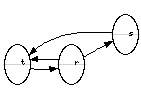
\includegraphics{model-01.png}

\begin{itemize}
\item $ \Re = (\{r,s,t\}, R) $
\item $ V(t) = \emptyset $ , $ V(s) = \{p,q\} $, $ V(r) = \{q\} $
\item $ \Phi := \square((p \rightarrow q) \wedge q ) $
\item Frage: Was l\"a\ss{}t sich \"uber die G\"ultigkeit von $ \Phi $ im gegebennen Model sagen?
\item Lsg: Bruteforce
  \begin{itemize}
  \item $ \Phi' := (p \rightarrow q) \wedge q \equiv (\neg p \vee q)\wedge q$
  \item Alle Welten untersuchen:
    \begin{itemize}
    \item $ M,r \models (p \rightarrow q) \wedge q \models (\neg p \vee q) \wedge q \rightarrow Wahr $
    \item $ M,s \models (\neg p \vee q ) \wedge q \rightarrow Wahr $
    \item $ M,t \models (\neg p \vee q ) \wedge q \rightarrow Falsch $
    \end{itemize}
  \item Frage stellen: Was ist erreichbar?
    \begin{itemize}
    \item $ M,r \models \square((p \rightarrow q ) \wedge q) $ gilt nicht (t von r aus erreichbar und in t gilt $ \Phi' $ nicht)
    \item $ M,s \models \square( \ldots ) $ ist falsch (von t aus s erreichbar und in t gilt $ \Phi' $ nicht)
    \item $ M,t \models \square( \ldots ) $ ist wahr (r einzige Folgewelt von t ist, $ \Phi' $ gilt)
    \end{itemize}
  \end{itemize}
\end{itemize}

\subsection{Graphen, Signaturen}
Es sei $ L = (E) $ die aus der Vorlsung beknnte Signatur der Graphen mit dem zweistelligen Relationssymbol E. Sei G ein beliebiges L-Model. Geben Sie L-Formeln $ \varphi_{1} $ und $ \varphi_{2} $ mit folgenden Eigenschaften an:
\begin{enumerate}
\item $ G \models \varphi_{1} \Leftrightarrow $ Der Graph G enth\"alt mindestens drei Knoten.
  \begin{itemize}
  \item $ \exists x_{1} \exists x_{2} \exists x_{3} (\neg x_{1} = x_{2} \wedge x_{1} = x3 \wedge \neg x_{2} = x_{2}) $
  \end{itemize}
\item $ G \models \varphi_{2} \Leftrightarrow $ Der Graph G enth\"alt h\"ochstens 3 Kanten.
  \begin{itemize}
  \item $ \neg $ ( G enth\"alt mindestens vier Kanten)
  \item $ \neg \exists x_{1} \ldots x_{8} ( x_{1}Ex_{2} \wedge x_{3}Ex_{4} \wedge x_{5}Ex_{6} \wedge x_{7}Ex_{8} \wedge (\neg x_{1} = x_{3} \vee \neg x_{2} = x_{4})
\wedge  (\neg x_{1} = x_{3} \vee \neg x_{2} = x_{4})
\wedge  (\neg x_{1} = x_{5} \vee \neg x_{2} = x_{6})
\wedge  (\neg x_{1} = x_{7} \vee \neg x_{2} = x_{8})
\wedge  (\neg x_{3} = x_{5} \vee \neg x_{4} = x_{6})
\wedge  (\neg x_{3} = x_{7} \vee \neg x_{4} = x_{8})
\wedge  (\neg x_{5} = x_{7} \vee \neg x_{6} = x_{8}))
$
  \end{itemize}
\end{enumerate}

\subsection{Partielle Ordnung ( $ \leq $ aka. PO )}
Es ist gegeben:
\begin{itemize}
\item $ \varphi_{1} := \forall x \forall y ( x \leq y \wedge \neg (x \leq y)) $
\item $ \varphi_{2} := \forall x \exists y \; x \leq y \wedge \forall y \exists x \; x \leq y $
\item $ \varphi_{3} := \exists x \forall y \; x \leq y $
\end{itemize}
F\"ur PO muss gelten:
\begin{enumerate}
\item $ \forall x \; x \leq x $
\item $ \forall x \forall y \; (x \leq y \wedge y \leq x \rightarrow x = y $
\item $ \forall x \forall y \forall z \; (x \leq y \wedge y \leq z \rightarrow x \leq z) $
\end{enumerate}

$ \Theta_{i} := \bigwedge^{i}_{j=1} \; \varphi_{j} $ f\"ur $ i = 1,2,3 \leftarrow $ allgemeing\"ulltig, erf\"ullbar, unwerfullbar

Lsg:
\begin{itemize}
\item $ \Theta_{1} = \varphi_{1} $ allgemeing\"ulltig : $  A \vee \neg A $ ist immer wahr
\item $ \Theta_{2} = \varphi_{1} \wedge \varphi_{2} $ allgemeing\"ulltig
\item $ \Theta_{3} = \varphi_{1} \wedge \varphi_{2} \wedge \varphi_{3} $ - erf\"ullbar
\end{itemize}

% You can even have references
\rule{0.3\linewidth}{0.25pt}
\scriptsize
\end{multicols}
\end{document}
